\documentclass[a4paper,11pt]{article}

\usepackage{etoolbox}
\usepackage{fancyvrb}
\usepackage[T1]{fontenc}
\usepackage{graphicx}
\usepackage{import}
\usepackage{listings}
%\usepackage{minted}
\usepackage{url}

\usepackage[
	% Prevent hyperlinks from getting an ugly border
    hidelinks,
    % Set proper PDF metadata
    pdftex,
    pdfauthor={Dennis Fischer},
    pdftitle={Detecting Process Memory Tampering},
    pdfsubject={TBD},
    pdfkeywords={dll injection, code injection, injection, code cave, nop, nop hopping, memory, tampering, detection, dll}
]{hyperref}
\usepackage{sections/_meta/tumlogo}

% Don't display "References" when rendering the bibliography
\patchcmd{\thebibliography}{\section*{\refname}}{}{}{}

% Use appropriate font size for line numbers in listings
\renewcommand{\theFancyVerbLine}{{\small\arabic{FancyVerbLine}}}

\lstset{basicstyle=\ttfamily}
\newcommand{\code}[1]{\texttt{#1}}

\setlength{\footnotesep}{0.4cm}
\setlength{\skip\footins}{0.5cm}

\def\doctype{Bachelor's Thesis in Informatics}
\def\title{Detecting Process Memory Tampering}
\def\germantitle{Erkennen von Prozess Speichermanipluationen}
\def\author{Dennis Fischer}
\def\date{Februar 15, 2016}

\begin{document}
\thispagestyle{empty}

\def\bcorcor{0.15cm}
\addtolength{\hoffset}{\bcorcor}

\thispagestyle{empty}

\vspace{4cm}

\begin{center}
  \oTUM{4cm}
  
  \vspace{5mm}
  
  \huge DEPARTMENT OF INFORMATICS\\
  
  \vspace{0.5cm}
  
  \large TECHNISCHE UNIVERSIT{\"A}T M{\"U}NCHEN\\
  
  \vspace{1mm}
\end{center}

\vspace{15mm}

\begin{center}
  {\Large \doctype}

  \vspace{20mm}

  \setlength\lineskip{8pt}
  {\LARGE \bf \title}\\%[3ex]

  \vspace{15mm}

  {\LARGE \author}

  \vspace{10mm}

  \begin{figure}[h!]
    \centering
    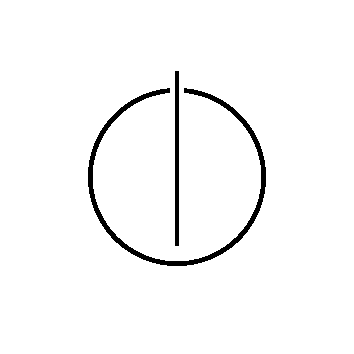
\includegraphics[width=4cm]{sections/_meta/informat.png}
  \end{figure}
\end{center}

\thispagestyle{empty}

\def\bcorcor{0.15cm}
\addtolength{\hoffset}{\bcorcor}

\thispagestyle{empty}

\vspace{4cm}

\begin{center}
  \oTUM{4cm}
  
  \vspace{5mm}
  
  \huge DEPARTMENT OF INFORMATICS\\
  
  \vspace{0.5cm}
  
  \large TECHNISCHE UNIVERSIT{\"A}T M{\"U}NCHEN\\
  
  \vspace{1mm}
\end{center}

\vspace{15mm}

\begin{center}
  {\Large \doctype}

  \vspace{20mm}

  \setlength\lineskip{8pt}
  {\LARGE \bf \title}\\%[3ex]

  \vspace{10mm}

  {\LARGE \germantitle}
\end{center}

\vfill

\renewcommand{\arraystretch}{0.7}

\begin{center}
\begin{tabular}{l@{\hskip 1cm}l}
  {\Large \bf Author:} & {\Large Dennis~Fischer} \\\\
  {\Large \bf Supervisor:} & {\Large Prof.~Dr.~Alexander~Pretschner} \\\\
  {\Large \bf Advisor:} & {\Large M.Sc.~Sebastian Banescu} \\\\
  {\Large \bf Submission date:} & {\Large 15.~Februar~2016}
\end{tabular}
\end{center}

\thispagestyle{empty}

\vspace*{\fill}
\begin{flushright}
\noindent \textit{I confirm that this bachelor's thesis is my own work \\ and I have documented all sources and material used.\\[\baselineskip]}
M{\"u}nchen, 15. Februar 2016 \\[3.5\baselineskip]
\underline{\hspace{6.5cm}}
\end{flushright}


\newpage
\thispagestyle{empty}
\null

% \newpage
\thispagestyle{empty}
\section*{Abstract}

TBD

\newpage
\pagestyle{empty}
\tableofcontents

\newpage
\pagestyle{plain}
\setcounter{page}{1}

\section{Motivation}

Many million users are using browsers daily to access internet pages and attackers are trying to make use of it, by using several different ways of attacking the browser itself. Often existing browser bugs (0-day exploits) or bugs in one of it's commonly used plugins like the Adobe Flash Player, to gain control of at least browser and often system functionalities. Another also very common way is the installation of unwanted toolbars without permissions by the controlling user. A possible way of doing so is dll-injection, which has been more commonly used in (online) game cheating, but can be used with arbitary applications to do malicious activities like openening and replacing ads or pishing techniques. This thesis will try to analyze the threads of Google Chrome's browser and do provenance of the existing threads, to detect unwanted dll-injections.
% PUT Content here!
\section{Design and Implementation}
The upcoming Design and Implementation chapter describes possible countermeasures to the previously shown attacks. The best working one is then being implemented.
\subsection{Requirements}
\subsection{Design and Architecture}
The attacks of Section \ref{sec:attacks} can be classified into two groups which have to be handled separately in order to increase security on the target platform. Attacks to the process virtual memory that have to use \gls{WPM}, which form the first group and attacks that are relying on a \gls{DLL} load during their initialization to execute their malicious code from inside, which form the second group. This classification makes it possible to design effective countermeasures that can not be avoided by attacks.

\begin{figure}[!htbp]
\centering
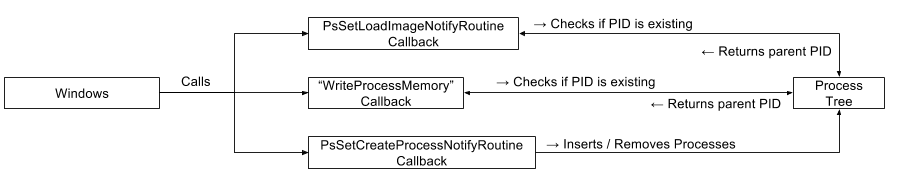
\includegraphics[angle=90,scale=0.6]{sections/implementation/interaction.png}
\caption{The interaction of the drivers components}
\label{fig:interaction}
\end{figure}

The classification into the two groups, \gls{DLL} and \gls{WPM}, is used to for the architecture design. Figure \ref{fig:interaction} shows the interacting components in an abstract representation. \emph{Windows} offers three entry points that will get called by the kernel, whenever a process is started, opened or a \gls{DLL} is loaded. The registered callback functions will then need to do several checks on the given information and based on this allow or deny execution.  
\paragraph{Process Tree Structure}
The \syscall{PsSetCreateProcessNotifyRoutine} callback function is called whenever a process is created or destroyed. Accordingly, whenever this callback function is executed, the process is inserted into the process tree structure on process creation, and removed from the process tree structure on process deletion. The process tree hereby maintains a list of lists, which is shown in Figure \ref{fig:listoflists}.
\begin{figure}[!htbp]
\centering
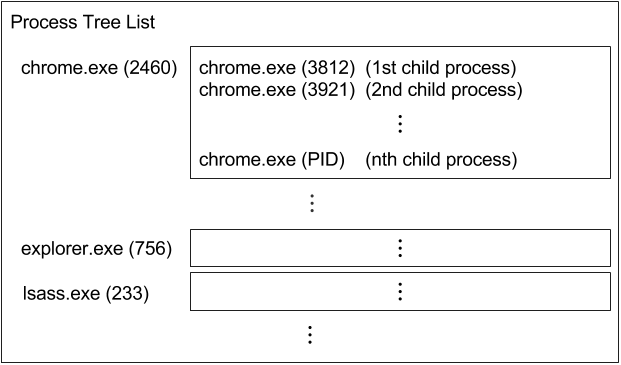
\includegraphics[scale=0.6]{sections/implementation/listoflists.png}
\caption{The process tree structure. A list of parent processes with their children}
\label{fig:listoflists}
\end{figure}
Each list separates the processes parents with their children from other processes. If the process tree gets queried for a specific \gls{PID} the parent \gls{PID} gets returned. To illustrate this interaction, the data of Figure \ref{fig:listoflists} is used for an example. If the process tree is queried with \gls{PID} 3812, a lookup in the process tree occurs to find a process with \gls{PID} 3812. In this case, the process is a child of chrome.exe with \gls{PID} 2460.
Because process 3812 is a child process, its parent 2460 is returned. For a second example, consider the process tree being queried for \gls{PID} 2460. Another lookup is done and a process with \gls{PID} 2460 is found. Because 2460 is a parent process, the process tree structure returns the value 2460.

\paragraph{DLL Component}
The last callback function of Figure \ref{fig:interaction}, \syscall{PsSetLoadImageNotifyRoutine}, is called by the \emph{Windows} kernel whenever a DLL is loaded. The callback routine queries the process tree structure for a given \gls{PID} to see if this is a chrome.exe process. If it is a chrome.exe process, the callback generates a hash of the DLL file, compares it to a whitelist and if a match can not be found takes action to prevent DLL loading.

\paragraph{WPM Component}
To prevent the group of \gls{WPM} attacks, a WPM callback is registered which checks if the given \gls{PID} is in a whitelist. If it is not, the request is denied by removing the required permissions to execute \gls{WPM} attacks. Because \glspl{PID} are dynamically assigned by the kernel and the possibility of reusing \glspl{PID}, a internal structure, a process tree, needs to be maintained. This thus adds communication between the three callback functions and the process tree as seen in Figure \ref{fig:interaction}.
\subsection{Implementation}
\label{sec:implementation} 

\subsection{Blocking \syscall{WriteProcessMemory} with a kernel mode driver}
The newly created problem with the modified \gls{ACL} can be solved by creating a driver running in kernel-mode. As reading memory, checking files and running processes are a common problem when writing anti virus software, Microsoft introduced object manager routines since Windows Vista to provide an efficient way of reacting onto these events. A driver will then use \syscall{ObRegisterCallbacks} to get notified whenever processes are created, files are opened and images (\glspl{DLL} and EXEs) are loaded. This functionality offers the programmer to create a pre- and post-execution callback function, that gets called whenever a process tries to receive a process handle. Microsoft offers an example driver using \syscall{ObRegisterCallbacks} at \cite{github_obcallback} and shows how to modify the requested process handle permissions to prevent termination by other applications such as the task manager. 

In order to protect chrome, the same actions described earlier will now be taken from inside the driver. Newly created process handles will be restricted to non virtual memory modifying permissions and the existing problem with inter process communication can be resolved by not restricting chromes child processes explicitly and giving them a full access handle. Appendix \ref{appendix:driver} shows an implemented driver to fulfill the requirements.

However, a naive implementation that just checks for process' executable file name may result in an access gain for the attacker. The injecting process simply has to be named chrome.exe and can gain access to the original chrome.exe. In this case, the implementation restricts outside access regardless of the given process name successfully. Children and parent \glspl{PID} are stored inside two separate tables that are on access checked if they contain target and source process ids. The driver is using a dynamic list structure, so that an unlimited number of processes can be tracked. Finally the check for access rights can be done by finding a given \gls{PID} inside the defined lists and returning a hash value, which uniquely identifies the process. 

A good hash for this tree is the parent \gls{PID}, as the process hierarchy is tracked inside the list. Only if both find operations result in a match of the returned \glspl{PID}, access is granted and no restriction is applied. Entries of the list (parent or child process) will get removed as soon as they exit, so that the remaining list is kept clean from garbage and reassignments of the same \gls{PID} do not lead to a security hole.

\subsection{Blocking DLL Injection with a kernel mode driver}
As previously stated, the resulting implementation already uses a kernel mode driver to prevent \gls{WPM} calls. It is therefore a suitable start point to prevent \gls{DLL} injections without being required to hook into the kernel. The Windows \gls{API} for drivers offers the \syscall{PsSetLoadImageNotfiyRoutine} function call, to register a callback function that is executed whenever a \gls{DLL} is mapped into memory. During the function call, the process is in a suspended state and thus execution of the \gls{DLL} has not begun. However, this entry point for \gls{DLL} load prevention is not optimal, as this function call occurs after the \gls{DLL} was already mapped into memory and a pre loading callback would be better to use in this situation. Unfortunately, this callback function does not exist so far, so the implementation has to rely on the post load callback.

To make use of \syscall{PsSetLoadImageNotifyRoutine}, the \gls{IRQL} may not be changed, because otherwise it can lead to a deadlock or even make the system crash in a blue screen of death. Most notably is the fact that the function call occurs on \gls{IRQL} \syscall{PASSIVE\_LEVEL} and special kernel mode \glspl{APC} are disabled. This is at first a major limitation to naive implementations. Opening and reading file calls will not complete, as the underlying \gls{APC} event is not sent, thus in a naive implementation, reading a file seems impossible at a first glance. The reason for the disabled special kernel mode \glspl{APC} is a previous call to the \syscall{KeEnterGuardedRegion} function, so a call to \syscall{KeLeaveGuardedRegion} can enable \gls{APC} events again. However, this should not be done here, as the result turns out to be unpredictable and leading to random deadlocks or failing accesses on files.

Having a deeper look at the windows kernel with a kernel debugger, a solution can be obtained by using a second running thread, a so called work item, which execution is handled separately by the system. The advantage of this are the enabled special kernel mode \glspl{APC} and the possibility to freely change the \gls{IRQL} during execution. One major disadvantage of this way is, that some sort of thread synchronization between the work item and the initial callback function has to be introduced and thus resulting into driver typical busy waiting, which is still faster than non busy waiting and eventually occurring context changes. 

A file handle can now be obtained and from the file data a sha256 \cite{eckert2014sicherheit} hash is generated, which is used later to compare it to a known whitelist of \gls{DLL} files. The Windows \gls{API} offers several different ways of obtaining a valid file handle with functions like \syscall{ZwOpenFile} or \syscall{ObOpenObjectByPointer}. The second function \syscall{ObOpenObjectByPointer} will generate a handle from a given pointer to an object. That is exactly what can be found inside the input parameters of the \syscall{PsSetLoadImageNotifyRoutine} callback. The image info can be extended to obtain a file object, and the \syscall{ObOpenObjectByPointer} function can then be used to obtain a handle from this file object. Though, this did not work in all cases and lead to \emph{random} results. 

If a file was opened a first time, \syscall{ObOpenObjectByPointer} will succeed and return a valid file handle. Subsequent calls to the same file lead to error \syscall{STATUS\_UNSUCCESSFUL} for no obvious reason. Kernel-debugging allowed to find the reason of failure, which is an internal call to \syscall{ObpIncrementHandleCount} that returns \syscall{STATUS\_UNSUCCESFUL}. There can be found nothing with respect to this problem and it might be a bug inside the windows kernel itself. 

Therefore, \syscall{ObOpenObjectByPointer} can not be used and only \syscall{ZwOpenFile} works as expected, but gives a new problem, the full file path. Path constructions is required, but will overall work and allow reading of all loaded \gls{DLL} files. Finally, the resulting sha256 hash can be calculated and compared to the whitelist and if no match is found, actions can be taken to prevent the \gls{DLL} from executing. 

An initial thought could be to undo the internal \syscall{ZwMapViewOfSection}/\syscall{NtMapViewOfSection} function that loaded the \gls{DLL} into memory by calling its counter pair \syscall{ZwUnmapViewOfSection}/\syscall{NtUnmapViewOfSection} and thus removing the \gls{DLL} from memory. The idea is great, but will not succeed as a special lock is hold, the LdrLoadLoaderLock, that can not be accessed at this point of code. Calling the functions regardless will deadlock the driver and soon after deadlock the whole system.

Thus, the \gls{DLL} will only get patched, rendering it, although still residing in memory, useless. To do that, three points in memory receive modifications: the entry point address, the \syscall{DOS MZ header}, which describes the file format of a \gls{DLL} with many meta information and the entry point function. The entry point address is set to \syscall{NULL}, the entry point function will get patched with a single \syscall{ret} (0xC3) instruction to prevent execution and the memory containing the \syscall{DOS MZ header} will get zeroed. All three steps guarantee, that nothing will be able to execute from this memory mapped \gls{DLL} file and thus preventing the typical \gls{DLL} injections from \syscall{SetWindowsHookEx}, the registry or other techniques.

% References
\section{References}
\bibliography{references}
\bibliographystyle{plain}
% PUT Appendix here!

\end{document}
